\documentclass[11pt,a4paper]{article}
\usepackage{bbm,amsthm,amsfonts,amssymb,amsmath,latexsym,epic,eepic}
\usepackage{marvosym,graphicx,fancyhdr,bbm}
\usepackage{graphicx}
\usepackage{color}
\usepackage[rflt]{floatflt}
\usepackage{colortbl}
\definecolor{Grey}{rgb}{0.5,0.5,0.5}
\definecolor{Red}{rgb}{1.0,0.0,0.0}

\usepackage{typearea}
\areaset{156mm}{235mm}
%\setlength{\parskip}{5pt plus 2pt minus 1pt}
\setlength{\parindent}{0pt}

% use \M for matrices and \V for vectors in math mode
\newcommand{\M}[1]{\mathbf{#1}}
\newcommand{\V}[1]{\mathbf{#1}}
\newcommand{\norm}[1]{\left | \left | #1 \right | \right |}
\newcommand{\RR}{\mathbbm{R}}        % set of real numbers


\renewcommand\floatpagefraction{0.8}
\renewcommand\topfraction{1}
\renewcommand\bottomfraction{0.9}
\renewcommand\textfraction{0.0}
%\def\dbltopfraction{1.0}
%\def\bottomfraction{1.0}
%\def\dblfloatpagefraction{0.8}


\makeatletter
\renewenvironment{thebibliography}[1]
     {\section*{\refname}%
      \@mkboth{\MakeUppercase\refname}{\MakeUppercase\refname}%
	 \parsep0mm
	 \itemsep0mm
	 %\labelsep0mm
	 %\itemindent0mm
      \list{\@biblabel{\@arabic\c@enumiv}}%
           {\settowidth\labelwidth{\@biblabel{#1}}%
            \leftmargin\labelwidth
            \advance\leftmargin\labelsep
            \@openbib@code
            \usecounter{enumiv}%
            \let\p@enumiv\@empty
            \renewcommand\theenumiv{\@arabic\c@enumiv}}%
      \sloppy
      \clubpenalty4000
      \@clubpenalty \clubpenalty
      \widowpenalty4000%
      \sfcode`\.\@m}
     {\def\@noitemerr
       {\@latex@warning{Empty `thebibliography' environment}}%
      \endlist}
\renewcommand\newblock{\hskip .11em\@plus.33em\@minus.07em}
\let\@openbib@code\@empty
\makeatother



\begin{document}\sloppy

\title{\Large\bf Vergleich der Pfadverfolgung mit Odometrie und AMCL \footnotetext{Diese Arbeit ist Bestandteil des Praktikums zur Mess- und Regelungstechnik}}

\author{Kai Hofmann und Barbara Fischbach\\
  Robotik und Telematik \\
  Universit\"at W\"urzburg\\
  Am Hubland, D-97074 W\"urzburg\\
{\small \texttt{barbara.fischbach@uni-wuerzburg.de}}\\
{\small \texttt{kai.hofmann@uni-wuerzburg.de}}}

\date{}




\maketitle

\newpage

\tableofcontents{}

\newpage

\twocolumn

\section*{Abstract}
\addcontentsline{toc}{section}{Abstract}
{
\textbf{Die autononome Fortbewegung von Fahrzeugen spielt heutzutage immer eine gr\"o\ss{}ere Rolle. Dazu werden verschiedene Algorithmen, zur Lokalisierung, Kartierung, und Pfadverfolgung genutzt. Diese wurden auf einem realen Roboter implementiert und getestet. Nicht nur im Weltall, wo wir unbedingt darauf angewiesen sind, dass Systeme autonom funktionieren, sondern auch auf der Erde, um Systeme sicherer und bequemer f\"ur den Benutzer zu machen. }


\section{Einleitung}
Um das überaus komplexe Thema verst\"andlicher zu machen und Algorithmen vorstellbar zu erkl\"aren, wird im folgenden ein Fraunhofer-Roboter benutzt, der anhand Odometrie,... sich selbst\"andig in einem bekannten Raum zurechtfinden kann.

\section{ROS}
F\"ur die Implementierung und Tests der Algorithmen wird das \textit{Robot Operating System}, kurz ROS genutzt. Es ist kein Betriebssystem im eigentlichen Sinn, sondern ein Framework. Es erm\"oglicht Hardware-Abstraktion, Paket-Managment und stellt eine Middleware bereit mit der verschiedene Prozesse kommunizieren k\"onnen. \cite{rosWiki}
Die ROS-Software ist in sogenannten Nodes organisiert, die über ROS miteienader kommunizieren k\"onnen. So können Funktionalitäten wie Plannung, Pfadverfolgung, Sensorik und so weiter getrennt werden. Außerdem können so einfach Nodes von anderen Leuten genutzt werden. Dies ermöglicht uns schnell eine Plattform zum testen der Algortithmen aufzubauen, und einfach Algorithmen durch Nodes zu implementieren 
 

\section{Lokalisation}
\subsection{Odometrie}
{Die Odometrie beruht auf einer relativen Positionsbestimmung, dabei wird aus der vorher bekannten Position und der zur\"uckgelegten Weg-strecke die neue Position berechnet. Auf kurzen Distanzen liefert die Odometrie sehr genaue Ergebnisse. Mit wachsender Entfernung nehmen auch Fehler durch unterschiedliche Dr\"ucke in den Reifen oder Reibung zu. Weitere Fehlerquelle sind h\"oheren Geschwindigkeiten und engeren Kurven, dort neigen die R\"ader zum Durchdrehen und Wegrutschen. Um das zu zeigen wird der Roboter \"ahnliche Pfade in langsamer und schneller Geschwindigkeit abfahren. 
	(Verkrüppeltes Bild einfügen)
	
	}
\subsection{Adaptive  Monte Carlo Localisation}
Im folgenden als AMCL abgek\"urzt, ist ein Algorithmus zur Lokalisation von Robotern. Dazu ben\"otigt der Roboter eine Karte der Umgebung. Der Roboter stellt Hypothesen über seine Pose auf der Karte an. Die anfägliche Verteilung dieser Hypothesen auf der Karte kann verschieden sein. 
Bei uns ist sie Gauß-verteilt um eine vom Menschen gegebene anfängliche Pose. 

\begin{figure}[h]
	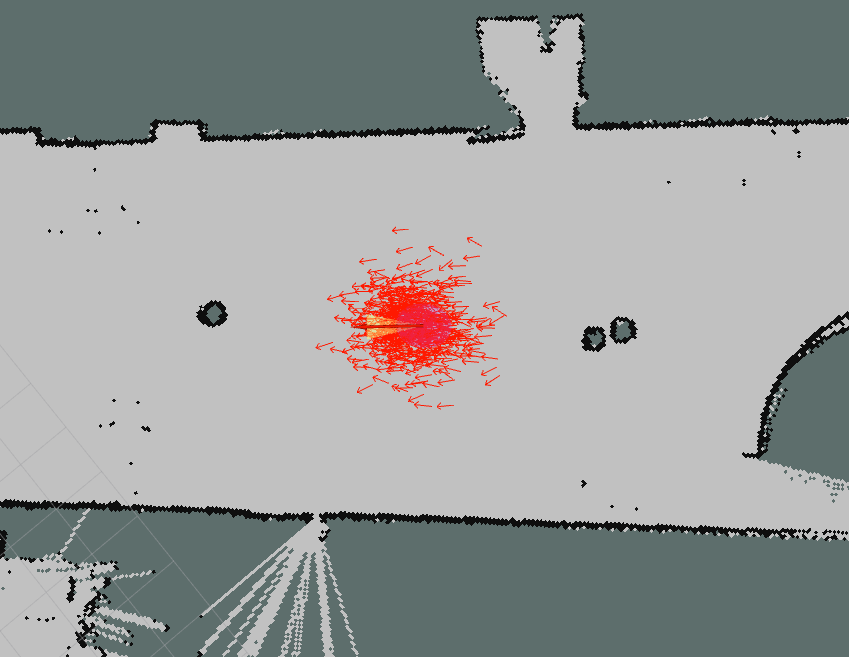
\includegraphics[width=\linewidth]{pictures/initial_distribution.jpg}
	\caption{Partikelverteilung in Anfangspose}
\end{figure}

Die Hypothesen kann man sich als virtuelle Roboter auf der Karte vorstellen. Fährt der reale Roboter, so fahren auch die virtuellen Roboter, mit den gleichen Steuerungsbefehlen. Die realen Sensorwerte werden mit denen der virtuellen Robotern verglichen. Die virtuellen Roboter gewinnen Ihre Sensormesswerte durch die Karte.

Je unstimmiger die Daten des virtuellen Roboters sind, desto unwahrscheinlicher ist die Hypothese dass der reale sich dort befindet. 

Unwahrscheinlichere Hypothesen werden gelöscht und neue im Bereich der wahrscheinlicheren aufgestellt, bzw. dort neue virtuelle Roboter erzeugt.

\begin{figure}[h]
	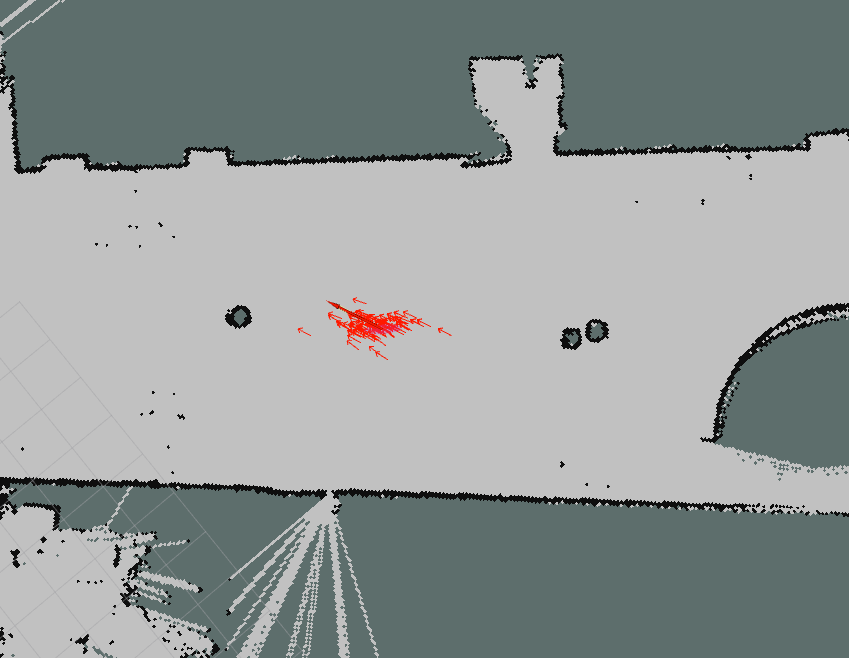
\includegraphics[width=\linewidth]{pictures/drive_little.jpg}
	\caption{Partikelverteilung nach kurzer Neuorientrierung durch Bewegung}
\end{figure}
 
Der virtuelle Roboter  mit besten den Übereinstimmungen, ist die beste Estimation der Pose.
Je näher die wahrscheinliche Hypothesen bei einander sind desto sicherer ist der Roboter sich seiner Pose. Dann kann die Anzahl der Hypothesen reduziert werden, daher dasss A wie Adaptive aus AMCL. Dies reduziert die CPU Auslastung und den Speicher

Partikel und Gewicht und Partikelfiler erwähnen, virtuelle Roboter nur in einem Satz erwähnen.

 


\subsection{Odometrie und AMCL im Vergleich}
Um die Lokalisation durch AMCL und Odometrie miteinander zu vergleichen f\"ahrt der Roboter einen "Acht"-f\"ormigen Pfad ab. Die Steuerung erfolgt manuell.  

->insert Diagramm mit Position durch Odometrie und AMCL 


Man erkennt folgende Unterschiede ...

Vorteil AMCL: Fehler summieren sich nicht auf (auch bei sehr langen Pfaden ist der Fehler nicht größer als er auch bei einem kürzen ist)
Nachteil AMCL: benötigt Karte, Pfad kann nicht in unbekannter Umgebung abgefahren werden

Nachteil Odmetrie: Aufsummation der Fehler bei langer Laufzeit , zunehmend schlechtere Qualität.
Vorteil: Odometrie in Echtzeit


\section{Kartierung mit Gmapping} \cite{gmapping}
Die Lokalisation eines Roboters ben\"otigt eine Karte. Eine unbekannte Umgebung wird aus den Daten eines Laserscanners und den aktuellen Posedaten erfasst und von dem Algorithmus GMapping verarbeitet. Die Posedaten publiziert die Odometrie an das ROS Paket gmapping.
Die Herausforderung liegt dabei in der gleichzeitigen Lokalisierung und Kartierung, dem \textit{simultaneous localization and mapping} Problem kurz SLAM. Denn beide bedingen sich gegenseitig. Um zum Beispiel zwei Laserscans zu einer Karte zusammenzuf\"ugen, m\"ussen die relativen Posen der Aufnahmen bekannt sein. Also ein Lokalisierungsproblem. Und um sich mit dem Laserscanner zu lokalisieren, benötigt man wiederum Kartendaten. 



g von Gmapping erklären!


Bild von der Karte einfügen

Das Untergeschoss des Informatikinstituts ist mit einem Roboter, der mit einem Sick-Laserscanner ausgestattet ist, in einer 2D-Karte kartiert.  Um diese Karte korrekt aufzunehmen werden nur so und soviel Partikel ben\"otigt. Die Aufnahme ist bis auf einen 1 cm genau und zeigt keine signifikanten Fehler. Bewegte Objekte wie Menschen werden erkannt und nicht in der Karte verzeichnet. Dagegen sorgt helles Licht, das durch die Fensterfronten scheint f\"ur eine Ungenauigkeit und kann nicht als klare Begrenzung festgestellt werden.
(Bild einfügen, in dem man Ungenauigkeit an Fenster sieht!) F\"ur klare Linie wie W\"ande ist es wichtig, das Gel\"ande mit einem Geschwindgkeitslimit von 1 m/s abzufahren. (Eventuell unsere erste Karte mit Dorits vergleichen?)

\begin{figure}[h]
	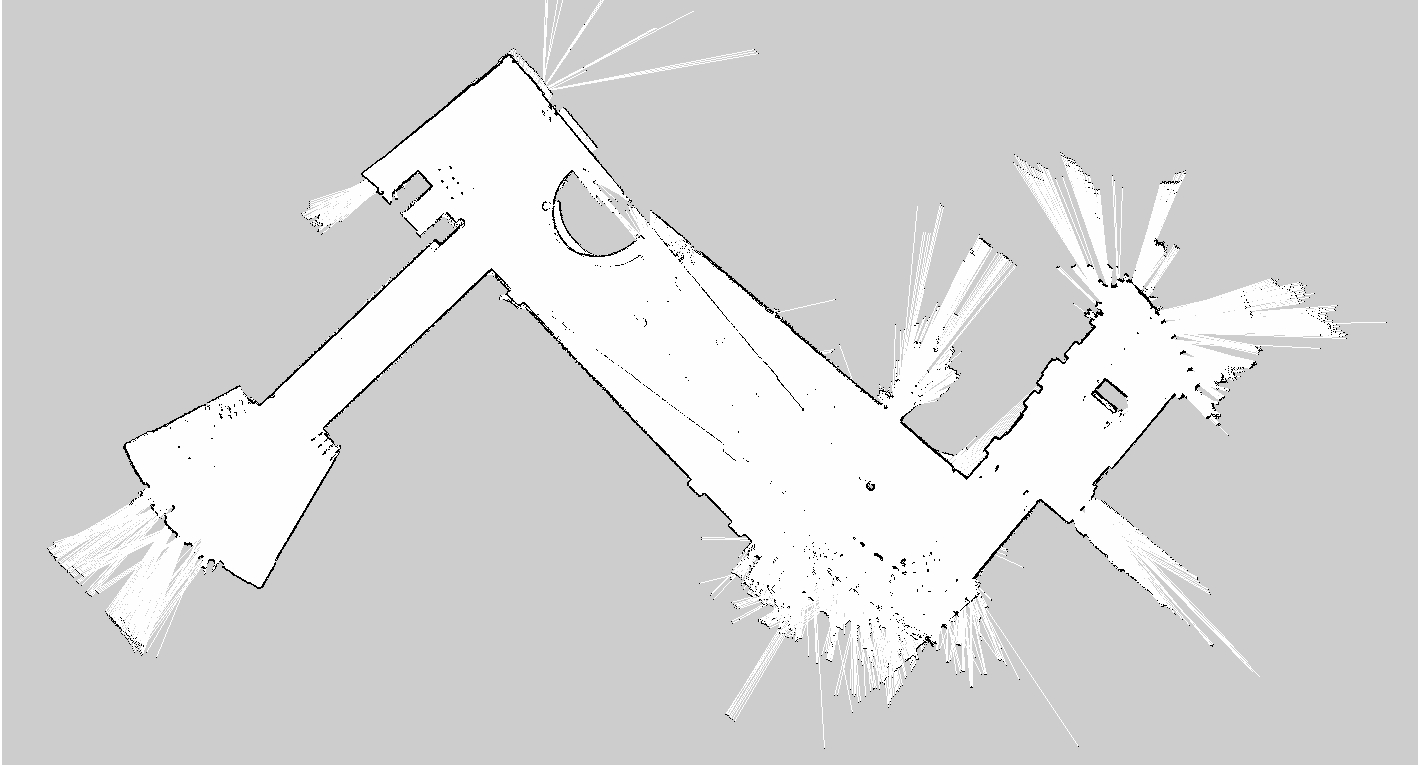
\includegraphics[width=0.5\textwidth]{pictures/firstMap.jpeg}
	\caption{Erkennbare Ungenauigkeiten durch Fenster und schr\"age Wand wegen zu hoher Geschwindigkeit}
\end{figure}


eigene Karte einfügen. AMCL erwähnen.


\section{Pfadverfolgung mit Giovanni Indiveri}
\cite{Giovanni}

Bild mit Pfad und Bezeichnungen einfügen

Der nicht-lineare Regler des Giovanni Indiveri und der Maria L. Corradini wird zur Pfadverfolgung verwendet. Die Implementierung garantiert nach Lyapunov, f\"ur einen beschr\"ankten, nicht-linearen Pfad, asymptotische Konvergenz und asymptotisch stabile Fehlerdynamik. Schrittweise neue Berechnungen der Reglerparameter f\"uhren zu schnelleren Konvergenz. Hierzu verwendet der Algorithmus eine orthogonale Projektion auf den Roboter selbst. Der Pfad wird zur Vereinfachungen in lineare Teilschnitte gen\"ahert, wodurch sich die Gleichungen vereinfachen.

Formeln aus Paper einfügen und Koordinatensystem

Durch Koordinatentransformation, dient die x-Achse als die Fahrtrichtung des Robotors  und y (der Roboter-Pfad-Abstand) \"ubernimmt die Rolle des l. Der Winkel Theta wird durch das \"ubereinanderlegen zu null.
Steering-Controll-Law vereinfacht sich...


\section{Zusammenfassung und Ausblick}


\newpage
{%\small                   % use small if you need it
	\bibliographystyle{plain}
	\bibliography{paper}       % use a bib-file paper.bib to collect

\end{document}



